\section{Background}
\label{sec:background}
The Blockchain is implemented as a chain of blocks where each one contains transactions. Blocks are created by users who are willing to use hardware resources in order to solve a computationally expensive mathematical problem which is unique for each block. Those users are called miners and once they verify the creation of a new block, the contained transactions are automatically approved and they get in return as a reward some Bitcoins. A block contains more than 500 transactions on average and its size can go up to 8MBs~\cite{damcosset}. 

The public nature of the Bitcoin Blockchain allows everyone to access the
complete history from the start and extract useful information. For instance,
one can indetify correlation patterns and trends or analyze the structure
evolution of the transactions graph, similar to our work. In the rest of this
section we provide some insight about the block and transaction schema as well as the
definitions of the metrics that we are going to compute for the transactions
graph.

\subsection{Block}
Every block in the Bitcoin network has the structure that ~\fref{fig:fig1} demonstrates. Each newly created block is chained to the last added and stores its digital fingerprint. The schema of the block is as follows:

\begin{itemize}
\item \textbf{Magic number (4 bytes):} This is an identifier for the Blockchain network. It has a constant value of 0xD9B4BEF9. It indicates the start of the block and that the data is from production network~\cite{medium}.

\item \textbf{Block size(4 bytes):} Indicates how large the block is.

\item \textbf{Version (4 bytes):} Mentions the Bitcoin protocol version that each node running on the network has to implement.

\item \textbf{Previous block hash (32 bytes):} It is a digital fingerprint (hash) of the \textit{block header} of the previous (last added) block of the Blockchain.

\item \textbf{Merkle Root (32 bytes):} A cryptographic hash of all of the transactions included in a block~\cite{architecture}.

\item \textbf{Timestamp (4 bytes):} The creation time of the block.

\item \textbf{Difficulty Target (4 bytes):} The current difficulty that was used to create this block.

\item \textbf{Nonce (4 bytes):} A random value that the creator of a block is allowed to manipulate.

\item \textbf{Transaction Counter (Variable: 1–9 bytes):} The number of transactions that are included within the block.

\item \textbf{Transaction List (Variable: Total block size is 1 MB):} Stores the digital fingerprint of all the transactions in that block.
\end{itemize}

Each block is characterized by a header. The \textit{Block header} is 80 bytes and it is composed by the fields from Version to Nonce.

\begin{figure}[htb]
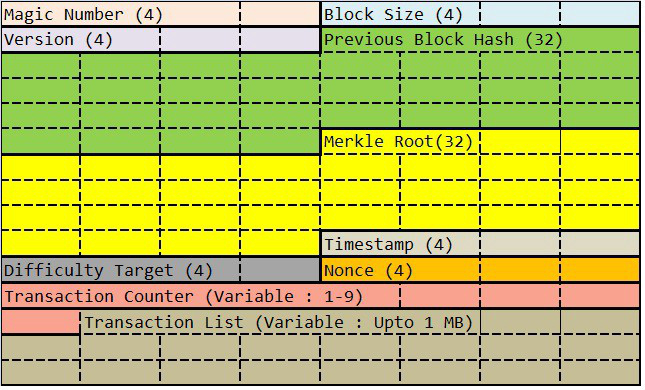
\includegraphics[width=1\linewidth]{./images/fig1}
\centering
\caption{The block structure. The number in the brackets is the size in bytes. Each individual cell is 1 byte. Hence, a field of 4 bytes occupies 4 cells. The fields from Version till Nonce are 80 bytes in total and form the \textit{block header}. Image source~\cite{medium}.}
\label{fig:fig1}
\end{figure}



\subsection{Transaction}
A Bitcoin transaction is the transfer or \textit{Bitcoins} from one address to another. Transferring does not mean physically moving an object from a source to a destination, but rather adding a new publicly accepted transaction entry to a block. Once a transaction is approved, it can never be removed or modified by anyone.

Transactions contain one-or-more inputs and one-or-more outputs. An \textit{input} is a reference to an output from a transaction in a previous block, whereas an \textit{output} specifies an amount and a address. Below we provide the abstract format of a Bitcoin transaction~\cite{mastering}:

\begin{itemize}
\item \textbf{Version (4 bytes):} Specifies which rules this transaction follows.
\item \textbf{Input Counter (1–9 bytes):} How many inputs are included.
\item \textbf{Inputs:} One or more transaction inputs.
\item \textbf{Output Counter (1–9 bytes):} How many outputs are included.
\item \textbf{Outputs:} One or more transaction outputs.
\item \textbf{Locktime (4 bytes):} A Unix timestamp or the block number.
\end{itemize}



\subsection{Metrics}
\label{label:metrics} The Bitcoin transactions can form a temporal graph in
which the transactions represent the edges of the graph and the Bitcoin
addresses represent the vertices. Based on this, we analyze the graph for each
year by computing some metrics that will provide us with an overall indication
of the structure. Below we provide the mathematical definition of each metric
that we compute later (Size, Triangle Participation Ratio, Bridge Ratio,
Clustering Coefficient, Conductance, Diameter) as well as the actual
information that these metrics provide for the structure of a graph in general.


\subsubsection{Size}
The size of the graph represents how big is the graph. It is the count of its total edges. In the following definition, ${\textstyle E}$ denotes the edges of the graph. 
\begin{align*}
  Sz &= \vert E \vert\\
\end{align*}



\subsubsection{Triangle Participation Ratio}
Triangle Participation Ratio (TPR) is a metric that for each vertex counts in how many triangles it participates in. In the following definition ${\textstyle t(x,S)}$ is the number of triangles that vertex ${\textstyle x}$ closes with-and-only-with the vertices in set ${\textstyle S}$.

\begin{align*}
  TPR &= \frac{\vert{\{x\in S : t(x,S) > 0 \}}\vert}{\vert S\vert}\\
\end{align*}



\subsubsection{Clustering Coefficient}
Clustering Coefficient is the measure of the degree to which nodes tend to cluster together. Three versions exist: the Global, the Local and the Average~\cite{cc}. 

Global Clustering Coefficient is designed to give an overall indication of the clustering in the network. In the following definition ${\textstyle tri(G)}$ is the number of triangles of a graph and ${\textstyle t(G)}$ is the number of the open and closed triplets.
\begin{align*}
  G\_CC &= \frac{ 3 \times tri(G) }{ t(G) }\\
\end{align*}

Local Clustering Coefficient provides an indication of the embeddedness of single nodes. It quantifies how close the neighbours of a vertex are to being a clique (complete graph). The Local Clustering Coefficient for a vertex ${\textstyle v_i}$ is given by the proportion of links between the vertices within its neighbourhood divided by the number of links that could possibly exist between them. For a directed graph, ${\textstyle e_{ij}}$ is distinct from ${\textstyle e_{ji}}$,  and therefore for each neighbourhood ${\textstyle N_i}$ there are ${\textstyle k_i (k_i - 1)}$ links that could exist among the vertices within the neighbourhood. In the following definition ${\textstyle k_i}$ is the number of neighbours of a vertex and ${\textstyle E}$ represent the edges of the graph.
\begin{align*}
  L\_CC &= \frac{\vert{\{e_jk : v_j,v_k \in N_i ,e_jk \in E\}}\vert}{k_i (k_i - 1)}\\
\end{align*}

Average is the mean of the Local Clustering Coefficient of all the vertices ${\textstyle n}$. The definition is as follows:
\begin{align*}
  \overline{L\_CC} &= \frac{1}{n} \sum_{i=1}^{n} C_i\\
\end{align*}



\subsubsection{Conductance}
The Conductance measures how "well-knit" is the graph. It controls how fast a random walk on ${\textstyle G}$ converges to a uniform distribution. Low Conductance means good clustering for the graph. The Conductance of the whole graph is the minimum conductance of all the possible cuts. In the following definition the cut of the graph is ${\textstyle (S,\overline{S})}$ and ${\textstyle \alpha_{ij}}$ are the entries of the adjacency matrix.
\begin{align*}
 	C &= \displaystyle\min_{S \subseteq V} ( \frac{\sum_{i \in S,j \in \overline{S}} \alpha_{ij} }{\min ( \alpha (S), \alpha ( \overline{S} ) )} ) 
\end{align*}



\subsubsection{Bridge Ratio}
Bridge ratio is the fraction of bridges to the total number of edges and its purpose is to show the vulnerabilities of a graph. A bridge is defined as an edge whose deletion disconnects the graph. In the following definition ${\textstyle N(x)}$ is the set of neighbors of ${\textstyle x}$ and ${\textstyle S}$ the set of vertices.
\begin{align*}
  BR &= \frac{bridges(S)}{\sum_{\mkern-5mu x\in S \vert{N(x)\cap S}\vert}}\\
\end{align*}



\subsubsection{Diameter}
Diameter is another measurement for the structure of a graph. It measures the topological length or extent of a graph by counting the number of edges in the shortest path between the most distant vertices~\cite{diameter}. Diameter is the maximum from all the shortest paths. In the following definition ${\textstyle s(i, j)}$ is the number of edges in the shortest path from vertex ${\textstyle i}$ to vertex ${\textstyle j}$.
\begin{align*}
  D &= \max(s(i,j))\\
\end{align*}
